\documentclass[11pt,]{article}
\usepackage{lmodern}
\usepackage{amssymb,amsmath}
\usepackage{ifxetex,ifluatex}
\usepackage{fixltx2e} % provides \textsubscript
\ifnum 0\ifxetex 1\fi\ifluatex 1\fi=0 % if pdftex
  \usepackage[T1]{fontenc}
  \usepackage[utf8]{inputenc}
\else % if luatex or xelatex
  \ifxetex
    \usepackage{mathspec}
  \else
    \usepackage{fontspec}
  \fi
  \defaultfontfeatures{Ligatures=TeX,Scale=MatchLowercase}
\fi
% use upquote if available, for straight quotes in verbatim environments
\IfFileExists{upquote.sty}{\usepackage{upquote}}{}
% use microtype if available
\IfFileExists{microtype.sty}{%
\usepackage{microtype}
\UseMicrotypeSet[protrusion]{basicmath} % disable protrusion for tt fonts
}{}
\usepackage[margin=0.5in]{geometry}
\usepackage{hyperref}
\hypersetup{unicode=true,
            pdftitle={P6 Penultimate Analyses},
            pdfauthor={Ryan Larson},
            pdfborder={0 0 0},
            breaklinks=true}
\urlstyle{same}  % don't use monospace font for urls
\usepackage{graphicx,grffile}
\makeatletter
\def\maxwidth{\ifdim\Gin@nat@width>\linewidth\linewidth\else\Gin@nat@width\fi}
\def\maxheight{\ifdim\Gin@nat@height>\textheight\textheight\else\Gin@nat@height\fi}
\makeatother
% Scale images if necessary, so that they will not overflow the page
% margins by default, and it is still possible to overwrite the defaults
% using explicit options in \includegraphics[width, height, ...]{}
\setkeys{Gin}{width=\maxwidth,height=\maxheight,keepaspectratio}
\IfFileExists{parskip.sty}{%
\usepackage{parskip}
}{% else
\setlength{\parindent}{0pt}
\setlength{\parskip}{6pt plus 2pt minus 1pt}
}
\setlength{\emergencystretch}{3em}  % prevent overfull lines
\providecommand{\tightlist}{%
  \setlength{\itemsep}{0pt}\setlength{\parskip}{0pt}}
\setcounter{secnumdepth}{0}
% Redefines (sub)paragraphs to behave more like sections
\ifx\paragraph\undefined\else
\let\oldparagraph\paragraph
\renewcommand{\paragraph}[1]{\oldparagraph{#1}\mbox{}}
\fi
\ifx\subparagraph\undefined\else
\let\oldsubparagraph\subparagraph
\renewcommand{\subparagraph}[1]{\oldsubparagraph{#1}\mbox{}}
\fi

%%% Use protect on footnotes to avoid problems with footnotes in titles
\let\rmarkdownfootnote\footnote%
\def\footnote{\protect\rmarkdownfootnote}

%%% Change title format to be more compact
\usepackage{titling}

% Create subtitle command for use in maketitle
\newcommand{\subtitle}[1]{
  \posttitle{
    \begin{center}\large#1\end{center}
    }
}

\setlength{\droptitle}{-2em}

  \title{P6 Penultimate Analyses}
    \pretitle{\vspace{\droptitle}\centering\huge}
  \posttitle{\par}
    \author{Ryan Larson}
    \preauthor{\centering\large\emph}
  \postauthor{\par}
      \predate{\centering\large\emph}
  \postdate{\par}
    \date{12/22/2018}

\usepackage{pdflscape}
\newcommand{\blandscape}{\begin{landscape}}
\newcommand{\elandscape}{\end{landscape}}

\begin{document}
\maketitle

\begin{table}[!htbp] \centering 
  \caption{Unweighted Descriptive Statistics} 
  \label{} 
\begin{tabular}{@{\extracolsep{5pt}}lcccccccc} 
\\[-1.8ex]\hline \\[-1.8ex] 
Statistic & \multicolumn{1}{c}{N} & \multicolumn{1}{c}{Mean} & \multicolumn{1}{c}{St. Dev.} & \multicolumn{1}{c}{Min} & \multicolumn{1}{c}{Pctl(25)} & \multicolumn{1}{c}{Median} & \multicolumn{1}{c}{Pctl(75)} & \multicolumn{1}{c}{Max} \\ 
\hline \\[-1.8ex] 
Felony History Pct. & 1,150 & 4.275 & 1.718 & 1.200 & 3.030 & 3.960 & 5.188 & 12.340 \\ 
Not Employed Rate & 1,150 & 22.230 & 4.237 & 12.986 & 19.323 & 21.935 & 24.869 & 37.585 \\ 
Population Share 16-25 & 1,150 & 18.318 & 1.780 & 13.331 & 17.218 & 18.183 & 19.343 & 27.342 \\ 
Population Share 26-35 & 1,150 & 19.068 & 2.792 & 12.553 & 16.760 & 18.732 & 21.314 & 29.370 \\ 
Population Share 36-45 & 1,150 & 19.705 & 1.996 & 13.676 & 18.315 & 19.768 & 21.020 & 29.022 \\ 
Population Share 46-55 & 1,150 & 16.306 & 2.482 & 10.655 & 14.069 & 16.740 & 18.344 & 23.034 \\ 
Population Share 56-65 & 1,150 & 11.838 & 1.749 & 7.055 & 10.545 & 11.517 & 12.931 & 17.791 \\ 
Population Share 66+ & 1,150 & 14.764 & 2.117 & 5.395 & 13.761 & 14.937 & 15.928 & 20.551 \\ 
Bachelor's Degree Rate & 1,150 & 21.609 & 7.688 & 4.539 & 18.459 & 22.703 & 26.425 & 41.208 \\ 
Marriage Rate & 1,150 & 57.067 & 4.227 & 44.599 & 54.123 & 56.793 & 59.817 & 71.036 \\ 
Ovr. Unemployment Rate t & 1,150 & 5.505 & 1.780 & 2.219 & 4.282 & 5.229 & 6.376 & 14.523 \\ 
Ovr. Unemployment Rate t-1 & 1,150 & 5.391 & 1.643 & 2.219 & 4.259 & 5.206 & 6.307 & 13.243 \\ 
Ovr. Unemployment Rate t-2 & 1,150 & 5.320 & 1.553 & 2.219 & 4.250 & 5.180 & 6.224 & 13.287 \\ 
Ovr. Unemployment Rate t-3 & 1,150 & 5.394 & 1.624 & 2.219 & 4.267 & 5.210 & 6.291 & 13.287 \\ 
Self-Report Disability Rate & 1,150 & 6.229 & 1.624 & 2.565 & 5.099 & 6.003 & 7.154 & 12.952 \\ 
SSI Rate & 1,150 & 2.739 & 1.161 & 0.765 & 1.893 & 2.402 & 3.324 & 7.110 \\ 
Effective Wage & 1,150 & 5.190 & 1.166 & 3.350 & 4.250 & 5.150 & 5.750 & 8.550 \\ 
Mean TANF Maximum & 1,150 & 403.792 & 155.250 & 117.667 & 289.333 & 376.333 & 507.667 & 925.333 \\ 
Unemployment Compensation & 1,150 & 358.496 & 65.844 & 157.124 & 311.618 & 356.399 & 400.119 & 581.813 \\ 
\hline \\[-1.8ex] 
\end{tabular} 
\end{table}

\subsubsection{Spaghetti Plots}\label{spaghetti-plots}

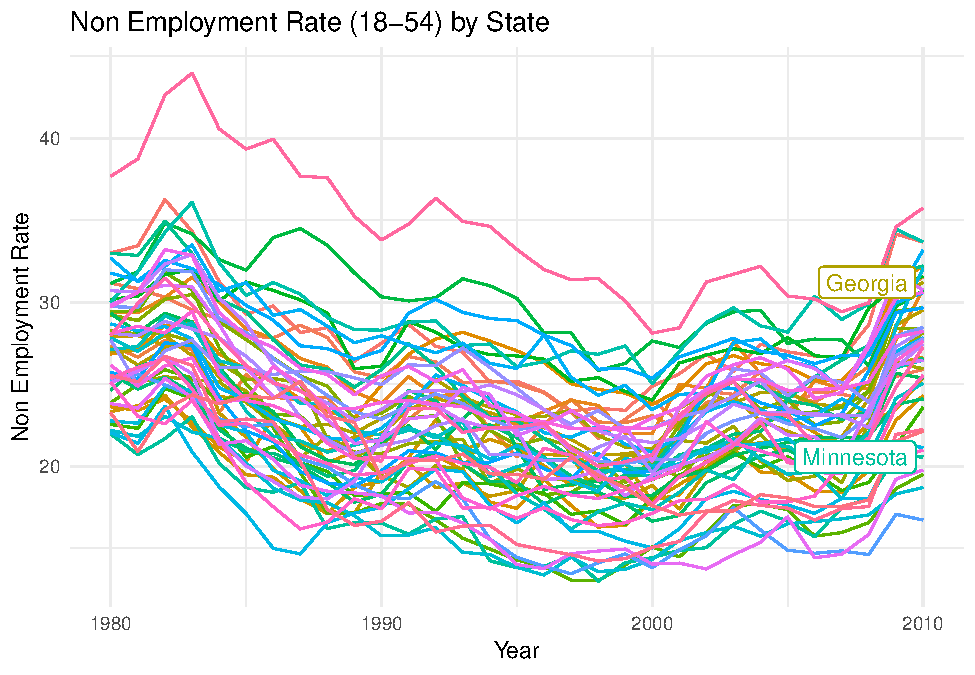
\includegraphics{P6_final_analyses_files/figure-latex/unnamed-chunk-3-1.pdf}

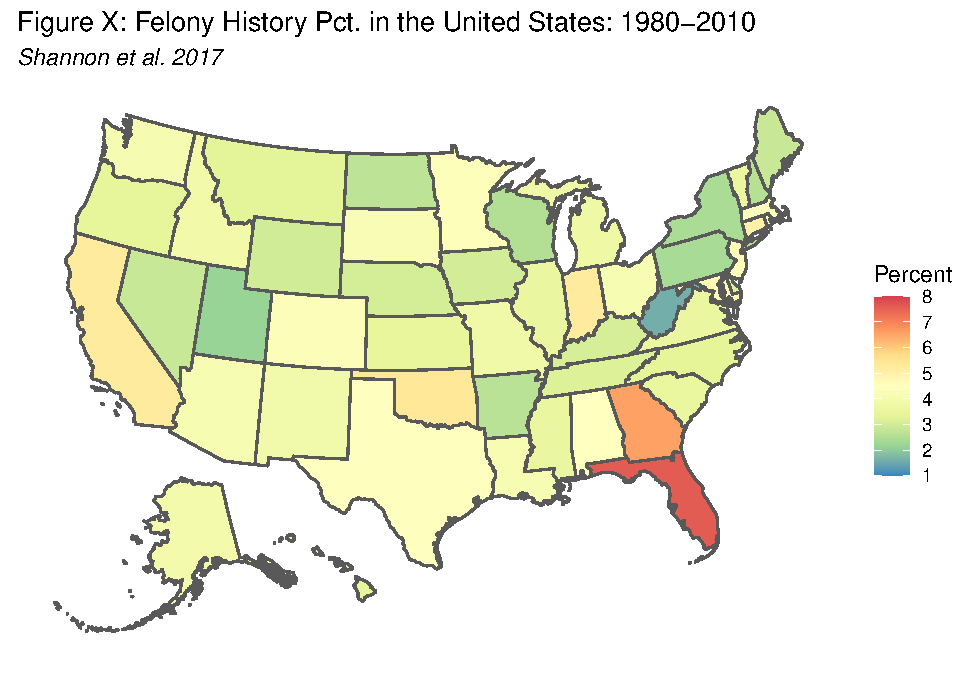
\includegraphics{P6_final_analyses_files/figure-latex/unnamed-chunk-4-1.pdf}

\subsubsection{p6 Overall Models}\label{p6-overall-models}

\begin{table}[!htbp] \centering 
  \caption{Panel Models of Not Employed Rate, 1988-2010} 
  \label{} 
\small 
\begin{tabular}{@{\extracolsep{5pt}}lD{.}{.}{-3} D{.}{.}{-3} D{.}{.}{-3} D{.}{.}{-3} } 
\\[-1.8ex]\hline 
\hline \\[-1.8ex] 
\\[-1.8ex] & \multicolumn{1}{c}{(1)} & \multicolumn{1}{c}{(2)} & \multicolumn{1}{c}{(3)} & \multicolumn{1}{c}{(4)}\\ 
\hline \\[-1.8ex] 
 Felony History Pct. & 0.319^{*}$ $(0.154) & 0.324^{*}$ $(0.157) & 0.304^{**}$ $(0.103) & 0.331^{***}$ $(0.100) \\ 
  Pop. Share 26-35 &  & 0.089$ $(0.078) & 0.060$ $(0.051) & 0.031$ $(0.052) \\ 
  Pop. Share 36-45 &  & 0.026$ $(0.077) & 0.067$ $(0.051) & 0.034$ $(0.050) \\ 
  Pop. Share 46-55 &  & 0.033$ $(0.076) & -0.081$ $(0.058) & -0.113$ $(0.058) \\ 
  Pop. Share 56-65 &  & 0.175$ $(0.095) & 0.153^{**}$ $(0.056) & 0.146^{**}$ $(0.055) \\ 
  Pop. Share 66+ &  & 0.084$ $(0.068) & 0.041$ $(0.048) & 0.012$ $(0.049) \\ 
  Degree Rate &  & 0.020$ $(0.038) & -0.055^{*}$ $(0.023) & -0.044^{*}$ $(0.022) \\ 
  Marriage Rate &  & -0.001$ $(0.044) & -0.007$ $(0.028) & 0.017$ $(0.027) \\ 
  Ovr. Unemp. Rate t &  &  & 0.892^{***}$ $(0.052) & 0.883^{***}$ $(0.050) \\ 
  Ovr. Unemp. Rate t-1 &  &  & 0.092^{*}$ $(0.037) & 0.101^{**}$ $(0.038) \\ 
  Ovr. Unemp. Rate t-2 &  &  & -0.016$ $(0.037) & -0.033$ $(0.037) \\ 
  Ovr. Unemp. Rate t-3 &  &  & 0.225^{***}$ $(0.038) & 0.220^{***}$ $(0.040) \\ 
  Disab. Rate &  &  &  & 0.149^{***}$ $(0.032) \\ 
  Effective Wage &  &  &  & -0.043$ $(0.109) \\ 
  Mean TANF Maximum &  &  &  & 0.000$ $(0.002) \\ 
  Unemployment Comp. &  &  &  & -0.000$ $(0.001) \\ 
 State FE & Yes & Yes & Yes & Yes \\ 
Year FE & Yes & Yes & Yes & Yes \\ 
Observations & \multicolumn{1}{c}{1,150} & \multicolumn{1}{c}{1,150} & \multicolumn{1}{c}{1,150} & \multicolumn{1}{c}{1,150} \\ 
R$^{2}$ & \multicolumn{1}{c}{0.015} & \multicolumn{1}{c}{0.008} & \multicolumn{1}{c}{0.566} & \multicolumn{1}{c}{0.574} \\ 
Adjusted R$^{2}$ & \multicolumn{1}{c}{-0.051} & \multicolumn{1}{c}{-0.065} & \multicolumn{1}{c}{0.532} & \multicolumn{1}{c}{0.539} \\ 
\hline \\[-1.8ex] 
\textit{Notes:} & \multicolumn{4}{l}{$^{***}$Significant at the 0.1 percent level.} \\ 
 & \multicolumn{4}{l}{$^{**}$Significant at the 1 percent level.} \\ 
 & \multicolumn{4}{l}{$^{*}$Significant at the 5 percent level.} \\ 
 & \multicolumn{4}{l}{Clustered Standard Errors by State and Year.} \\ 
 & \multicolumn{4}{l}{Weighted by State-Year total pop.} \\ 
\end{tabular} 
\end{table}

\pagebreak

\subsubsection{Robustness Checks}\label{robustness-checks}

\begin{table}[!htbp] \centering 
  \caption{Panel Models of Unemployment and Idleness Rates, 1988-2010} 
  \label{} 
\small 
\begin{tabular}{@{\extracolsep{5pt}}lD{.}{.}{-3} D{.}{.}{-3} } 
\\[-1.8ex]\hline 
\hline \\[-1.8ex] 
\\[-1.8ex] & \multicolumn{1}{c}{Unemployment} & \multicolumn{1}{c}{Idleness} \\ 
\\[-1.8ex] & \multicolumn{1}{c}{(1)} & \multicolumn{1}{c}{(2)}\\ 
\hline \\[-1.8ex] 
 Felony History Pct. & 0.010$ $(0.009) & 0.331^{***}$ $(0.099) \\ 
  Pop. Share 26-35 & 0.013^{*}$ $(0.005) & 0.050$ $(0.052) \\ 
  Pop. Share 36-45 & 0.019^{*}$ $(0.007) & 0.035$ $(0.051) \\ 
  Pop. Share 46-55 & 0.004$ $(0.006) & -0.116$ $(0.060) \\ 
  Pop. Share 56-65 & 0.005$ $(0.008) & 0.133^{*}$ $(0.054) \\ 
  Pop. Share 66+ & 0.015^{**}$ $(0.006) & 0.025$ $(0.050) \\ 
  Degree Rate & -0.008^{**}$ $(0.003) & -0.028$ $(0.022) \\ 
  Marriage Rate & -0.011^{***}$ $(0.002) & 0.030$ $(0.028) \\ 
  Ovr. Unemp. Rate t & 1.021^{***}$ $(0.008) & 0.086$ $(0.050) \\ 
  Ovr. Unemp. Rate t-1 & -0.001$ $(0.010) & 0.139^{***}$ $(0.038) \\ 
  Ovr. Unemp. Rate t-2 & -0.038^{***}$ $(0.008) & -0.041$ $(0.038) \\ 
  Ovr. Unemp. Rate t-3 & 0.022^{***}$ $(0.007) & 0.212^{***}$ $(0.040) \\ 
  Disab. Rate & 0.004$ $(0.004) & 0.157^{***}$ $(0.032) \\ 
  Effective Wage & 0.000$ $(0.018) & -0.038$ $(0.111) \\ 
  Mean TANF Maximum & 0.000$ $(0.000) & 0.000$ $(0.002) \\ 
  Unemployment Comp. & -0.000$ $(0.000) & 0.000$ $(0.001) \\ 
 State FE & Yes & Yes \\ 
Year FE & Yes & Yes \\ 
Observations & \multicolumn{1}{c}{1,150} & \multicolumn{1}{c}{1,150} \\ 
R$^{2}$ & \multicolumn{1}{c}{0.975} & \multicolumn{1}{c}{0.151} \\ 
Adjusted R$^{2}$ & \multicolumn{1}{c}{0.973} & \multicolumn{1}{c}{0.082} \\ 
\hline \\[-1.8ex] 
\textit{Notes:} & \multicolumn{2}{l}{$^{***}$Significant at the 0.1 percent level.} \\ 
 & \multicolumn{2}{l}{$^{**}$Significant at the 1 percent level.} \\ 
 & \multicolumn{2}{l}{$^{*}$Significant at the 5 percent level.} \\ 
 & \multicolumn{2}{l}{Clustered Standard Errors by State and Year.} \\ 
 & \multicolumn{2}{l}{Weighted by State-Year total pop.} \\ 
\end{tabular} 
\end{table}

\pagebreak

\section{Alternative Sample Models}\label{alternative-sample-models}

\begin{table}[!htbp] \centering 
  \caption{Alternative Sample Models} 
  \label{} 
\small 
\begin{tabular}{@{\extracolsep{5pt}}lD{.}{.}{-3} D{.}{.}{-3} D{.}{.}{-3} D{.}{.}{-3} } 
\\[-1.8ex]\hline 
\hline \\[-1.8ex] 
 & \multicolumn{1}{c}{Male} & \multicolumn{1}{c}{Female} & \multicolumn{1}{c}{Black} & \multicolumn{1}{c}{White} \\ 
\\[-1.8ex] & \multicolumn{1}{c}{(1)} & \multicolumn{1}{c}{(2)} & \multicolumn{1}{c}{(3)} & \multicolumn{1}{c}{(4)}\\ 
\hline \\[-1.8ex] 
 Felony History Pct. & 0.109$ $(0.088) & 0.555^{***}$ $(0.167) & 0.058$ $(0.058) & 0.406^{***}$ $(0.118) \\ 
  Pop. Share 26-35 & 0.082$ $(0.045) & 0.023$ $(0.074) & 0.333^{**}$ $(0.120) & 0.062$ $(0.054) \\ 
  Pop. Share 36-45 & 0.245^{***}$ $(0.052) & -0.099$ $(0.070) & 0.218$ $(0.118) & 0.103$ $(0.053) \\ 
  Pop. Share 46-55 & 0.062$ $(0.040) & -0.241^{*}$ $(0.099) & -0.127$ $(0.172) & -0.065$ $(0.068) \\ 
  Pop. Share 56-65 & 0.107^{*}$ $(0.049) & 0.178^{*}$ $(0.089) & 0.495^{**}$ $(0.170) & 0.172^{**}$ $(0.063) \\ 
  Pop. Share 66+ & 0.203^{***}$ $(0.046) & -0.131$ $(0.076) & 0.042$ $(0.120) & 0.051$ $(0.054) \\ 
  Degree Rate & 1.108^{***}$ $(0.049) & 0.670^{***}$ $(0.076) & 1.196^{***}$ $(0.122) & 0.850^{***}$ $(0.054) \\ 
  Marriage Rate & 0.109^{***}$ $(0.033) & 0.092$ $(0.059) & 0.005$ $(0.129) & 0.131^{**}$ $(0.040) \\ 
  Ovr. Unemp. Rate t & -0.021$ $(0.034) & -0.026$ $(0.058) & -0.001$ $(0.147) & -0.057$ $(0.040) \\ 
  Ovr. Unemp. Rate t-1 & 0.056$ $(0.031) & 0.373^{***}$ $(0.069) & 0.679^{***}$ $(0.125) & 0.115^{*}$ $(0.046) \\ 
  Ovr. Unemp. Rate t-2 & -0.008$ $(0.016) & -0.079^{*}$ $(0.038) & -0.089^{***}$ $(0.011) & -0.080^{***}$ $(0.022) \\ 
  Ovr. Unemp. Rate t-3 & -0.143^{***}$ $(0.022) & 0.107^{**}$ $(0.034) & -0.175^{***}$ $(0.009) & 0.015$ $(0.031) \\ 
  Disab. Rate & 0.180^{***}$ $(0.020) & 0.058$ $(0.048) & 0.155^{***}$ $(0.008) & 0.137^{***}$ $(0.034) \\ 
  Effective Wage & 0.218^{**}$ $(0.075) & -0.278$ $(0.201) & -0.535$ $(0.276) & 0.011$ $(0.129) \\ 
  Mean TANF Maximum & 0.001$ $(0.001) & -0.000$ $(0.003) & 0.004$ $(0.004) & -0.001$ $(0.002) \\ 
  Unemployment Comp. & -0.002$ $(0.001) & 0.002$ $(0.002) & -0.006$ $(0.004) & -0.000$ $(0.001) \\ 
  Disab. Imputed &  &  & 1.946^{***}$ $(0.317) &  \\ 
  Marriage Imputed &  &  & 13.639^{***}$ $(0.962) &  \\ 
 State FE & Yes & Yes & Yes & Yes \\ 
Year FE & Yes & Yes & Yes & Yes \\ 
Observations & \multicolumn{1}{c}{1,150} & \multicolumn{1}{c}{1,150} & \multicolumn{1}{c}{1,118} & \multicolumn{1}{c}{1,150} \\ 
R$^{2}$ & \multicolumn{1}{c}{0.608} & \multicolumn{1}{c}{0.335} & \multicolumn{1}{c}{0.068} & \multicolumn{1}{c}{0.514} \\ 
Adjusted R$^{2}$ & \multicolumn{1}{c}{0.576} & \multicolumn{1}{c}{0.280} & \multicolumn{1}{c}{-0.013} & \multicolumn{1}{c}{0.474} \\ 
\hline \\[-1.8ex] 
\textit{Notes:} & \multicolumn{4}{l}{$^{***}$Significant at the 0.1 percent level.} \\ 
 & \multicolumn{4}{l}{$^{**}$Significant at the 1 percent level.} \\ 
 & \multicolumn{4}{l}{$^{*}$Significant at the 5 percent level.} \\ 
 & \multicolumn{4}{l}{Clustered Standard Errors by State and Year.} \\ 
 & \multicolumn{4}{l}{Weighted by State-Year total pop.} \\ 
\end{tabular} 
\end{table}

\pagebreak

\pagebreak

\section{Alternative Specifications of
Disabiility}\label{alternative-specifications-of-disabiility}

\begin{table}[!htbp] \centering 
  \caption{Alternative Specifications of Disability} 
  \label{} 
\small 
\begin{tabular}{@{\extracolsep{5pt}}lccc} 
\\[-1.8ex]\hline 
\hline \\[-1.8ex] 
 & with SSI & Imputed & Imputed no SSI \\ 
\\[-1.8ex] & (1) & (2) & (3)\\ 
\hline \\[-1.8ex] 
 Felon History Pct. & 0.315$^{**}$ (0.099) & 0.321$^{***}$ (0.084) & 0.332$^{***}$ (0.088) \\ 
  Pop. Share 26-35 & 0.025 (0.051) & 0.042 (0.048) & 0.044 (0.049) \\ 
  Pop. Share 36-45 & 0.034 (0.049) & $-$0.013 (0.047) & $-$0.008 (0.048) \\ 
  Pop. Share 46-55 & $-$0.115$^{*}$ (0.057) & $-$0.197$^{**}$ (0.062) & $-$0.193$^{**}$ (0.062) \\ 
  Pop. Share 56-65 & 0.124$^{*}$ (0.053) & 0.057 (0.052) & 0.088 (0.054) \\ 
  Pop. Share 66+ & 0.019 (0.049) & 0.025 (0.050) & 0.017 (0.049) \\ 
  Degree Rate & 0.853$^{***}$ (0.050) & 0.918$^{***}$ (0.044) & 0.937$^{***}$ (0.044) \\ 
  Marriage Rate & 0.105$^{**}$ (0.038) & 0.084$^{**}$ (0.030) & 0.082$^{**}$ (0.029) \\ 
  Ovr. Unemp. Rate t & $-$0.026 (0.037) & $-$0.011 (0.026) & $-$0.015 (0.026) \\ 
  Ovr. Unemp. Rate t-1 & 0.217$^{***}$ (0.037) & 0.234$^{***}$ (0.043) & 0.236$^{***}$ (0.044) \\ 
  Ovr. Unemp. Rate t-2 & $-$0.046$^{*}$ (0.022) & $-$0.066$^{*}$ (0.026) & $-$0.066$^{*}$ (0.026) \\ 
  Ovr. Unemp. Rate t-3 & 0.018 (0.026) & 0.055$^{*}$ (0.025) & 0.051$^{*}$ (0.025) \\ 
  Disab.rate & 0.162$^{***}$ (0.030) & 0.165$^{***}$ (0.038) & 0.155$^{***}$ (0.038) \\ 
  SSI Rate & $-$0.487$^{*}$ (0.192) & $-$0.344 (0.198) &  \\ 
  Effective Wage & $-$0.002 (0.110) & 0.138 (0.119) & 0.107 (0.124) \\ 
  Mean TANF Maximum & 0.000 (0.002) & 0.001 (0.001) & 0.000 (0.001) \\ 
  Unemployment Comp. & $-$0.000 (0.001) & $-$0.001 (0.001) & $-$0.001 (0.001) \\ 
 State FE & Yes & Yes & Yes \\ 
Year FE & Yes & Yes & Yes \\ 
Observations & 1,150 & 1,400 & 1,400 \\ 
R$^{2}$ & 0.576 & 0.601 & 0.600 \\ 
Adjusted R$^{2}$ & 0.541 & 0.573 & 0.572 \\ 
\hline \\[-1.8ex] 
\textit{Notes:} & \multicolumn{3}{l}{$^{***}$Significant at the 0.1 percent level.} \\ 
 & \multicolumn{3}{l}{$^{**}$Significant at the 1 percent level.} \\ 
 & \multicolumn{3}{l}{$^{*}$Significant at the 5 percent level.} \\ 
 & \multicolumn{3}{l}{Clustered Standard Errors by State and Year.} \\ 
 & \multicolumn{3}{l}{Weighted by State-Year total pop.} \\ 
\end{tabular} 
\end{table}

\pagebreak

\section{Felon Density Maps}\label{felon-density-maps}

\includegraphics{P6_final_analyses_files/figure-latex/unnamed-chunk-14-1.pdf}

\pagebreak

\includegraphics{P6_final_analyses_files/figure-latex/unnamed-chunk-15-1.pdf}

\pagebreak

\includegraphics{P6_final_analyses_files/figure-latex/unnamed-chunk-16-1.pdf}

\begin{table}[!htbp] \centering 
  \caption{Pairwise Correlations} 
  \label{} 
\small 
\begin{tabular}{@{\extracolsep{0.15pt}} cccccccccccccccccccc} 
\\[-1.8ex]\hline 
\hline \\[-1.8ex] 
Variable & 1 & 2 & 3 & 4 & 5 & 6 & 7 & 8 & 9 & 10 & 11 & 12 & 13 & 14 & 15 & 16 & 17 & 18 & 19 \\ 
\hline \\[-1.8ex] 
Felony History Pct. & 1 &  &  &  &  &  &  &  &  &  &  &  &  &  &  &  &  &  &  \\ 
Not Employed Rate & 0.14 & 1 &  &  &  &  &  &  &  &  &  &  &  &  &  &  &  &  &  \\ 
Population Share 16-25 & -0.25 & 0 & 1 &  &  &  &  &  &  &  &  &  &  &  &  &  &  &  &  \\ 
Population Share 26-35 & -0.37 & -0.05 & 0.37 & 1 &  &  &  &  &  &  &  &  &  &  &  &  &  &  &  \\ 
Population Share 36-45 & -0.18 & -0.27 & -0.13 & 0.28 & 1 &  &  &  &  &  &  &  &  &  &  &  &  &  &  \\ 
Population Share 46-55 & 0.49 & 0.06 & -0.4 & -0.83 & -0.21 & 1 &  &  &  &  &  &  &  &  &  &  &  &  &  \\ 
Population Share 56-65 & 0.34 & 0.33 & -0.37 & -0.61 & -0.7 & 0.54 & 1 &  &  &  &  &  &  &  &  &  &  &  &  \\ 
Population Share 66+ & 0.01 & -0.02 & -0.43 & -0.42 & -0.38 & 0 & 0.32 & 1 &  &  &  &  &  &  &  &  &  &  &  \\ 
Bachelor's Degree Rate & 0.45 & -0.15 & -0.4 & -0.56 & 0.1 & 0.68 & 0.19 & 0.03 & 1 &  &  &  &  &  &  &  &  &  &  \\ 
Marriage Rate & -0.49 & -0.26 & 0.36 & 0.46 & 0.27 & -0.55 & -0.47 & -0.14 & -0.55 & 1 &  &  &  &  &  &  &  &  &  \\ 
Ovr. Unemployment Rate t & 0.11 & 0.76 & 0 & 0.06 & -0.2 & -0.01 & 0.23 & -0.07 & -0.1 & -0.22 & 1 &  &  &  &  &  &  &  &  \\ 
Ovr. Unemployment Rate t-1 & -0.01 & 0.69 & 0.06 & 0.18 & -0.07 & -0.13 & 0.06 & -0.1 & -0.16 & -0.07 & 0.82 & 1 &  &  &  &  &  &  &  \\ 
Ovr. Unemployment Rate t-2 & -0.15 & 0.55 & 0.13 & 0.32 & 0.07 & -0.28 & -0.14 & -0.15 & -0.31 & 0.14 & 0.51 & 0.79 & 1 &  &  &  &  &  &  \\ 
Ovr. Unemployment Rate t-3 & -0.21 & 0.46 & 0.14 & 0.35 & 0.09 & -0.32 & -0.18 & -0.14 & -0.4 & 0.21 & 0.33 & 0.57 & 0.88 & 1 &  &  &  &  &  \\ 
Self-Report Disability Rate & -0.04 & 0.47 & -0.22 & -0.31 & -0.09 & 0.21 & 0.24 & 0.23 & -0.05 & -0.1 & 0.25 & 0.28 & 0.29 & 0.27 & 1 &  &  &  &  \\ 
SSI Rate & 0.08 & 0.65 & -0.05 & -0.2 & -0.15 & 0.09 & 0.18 & 0.19 & -0.05 & -0.27 & 0.3 & 0.32 & 0.33 & 0.31 & 0.62 & 1 &  &  &  \\ 
Effective Wage & 0.54 & 0.19 & -0.32 & -0.69 & -0.34 & 0.78 & 0.62 & 0.06 & 0.65 & -0.64 & 0.23 & 0 & -0.28 & -0.34 & 0.11 & 0.11 & 1 &  &  \\ 
Mean TANF Maximum & 0.01 & -0.25 & -0.15 & -0.04 & 0.23 & 0.2 & -0.06 & -0.21 & 0.36 & -0.21 & -0.03 & -0.07 & -0.12 & -0.15 & -0.26 & -0.37 & 0.27 & 1 &  \\ 
Unemployment Compensation & 0.03 & 0.12 & -0.18 & -0.18 & -0.06 & 0.21 & 0.14 & 0.07 & 0.25 & -0.11 & 0.1 & 0.07 & 0.03 & 0 & 0.11 & 0.02 & 0.23 & 0.08 & 1 \\ 
\hline \\[-1.8ex] 
\end{tabular} 
\end{table}


\end{document}
